%% ICMRA 2026 -- 8th International Conference on Mechatronics, Robotics and Automation
%% IEEE conference format. Compile with pdflatex (IEEEtran class).
\documentclass[conference]{IEEEtran}
\IEEEoverridecommandlockouts

\usepackage{cite}
\usepackage{amsmath,amssymb}
\usepackage{graphicx}
\usepackage{booktabs}
\usepackage{url}
\usepackage[hidelinks]{hyperref}

\begin{document}

\title{From Cross-Facility Detection to Metric 3D Localisation:\\A Monocular Perception Pipeline for Robotic\\Electric Vehicle Battery Disassembly}

\author{\IEEEauthorblockN{Komiljon Qosimov}
\IEEEauthorblockA{\textit{School of Engineering} \\
\textit{University of Birmingham}\\
Birmingham, United Kingdom \\
kxk445@student.bham.ac.uk}
\and
\IEEEauthorblockN{Yujie Wang}
\IEEEauthorblockA{\textit{School of Engineering} \\
\textit{University of Birmingham}\\
Birmingham, United Kingdom}
}

\maketitle

\begin{abstract}
Robotic disassembly of end-of-life electric vehicle (EV) battery packs depends on
perception that works on packs a system has never seen. Published detectors are
almost always trained and evaluated on a single facility or a single rig, so their
reported accuracy does not indicate whether they will transfer. We quantify this gap
directly. A detector achieving 0.818 mAP@50 on the single-facility benchmark it was
trained on falls to 0.277 mAP@50 on a 225-image benchmark spanning ten independent
pack sources -- a 66\% relative loss. We then assemble a multi-source training set
(4,425 images, 13 sources, ten pack families) and compare a from-scratch YOLO11n
detector against RF-DETR, a real-time detection transformer with a frozen
self-supervised DINOv2 backbone. Under an identical evaluation protocol RF-DETR
attains 0.502 mAP@50 versus 0.410 for YOLO11n. Per-class analysis shows the two are
statistically indistinguishable on conventionally annotated packs (module 0.771 vs
0.774); the entire advantage arises from graceful degradation under
annotation-convention shift, where YOLO11n collapses (module 0.774 $\rightarrow$
0.547) and RF-DETR does not (0.771 $\rightarrow$ 0.680). We further identify
annotation convention as a measurable, dominant failure mode: per-source module
mAP@50 ranges from 0.995 to 0.043, with the low outlier explained entirely by a
divergent labelling definition rather than any visual difficulty. Finally, we show
that condition assessment can be performed without any damaged training examples: a
good-only anomaly detector over frozen DINOv2 patch features attains 0.857 recall on
damaged modules, matching a supervised classifier trained on scarce damaged data.
Finally, because a detection alone cannot command a manipulator, we close the loop to
metric 3D: a fiducial-referenced homography lifts 2D detections into robot-frame
coordinates from a single RGB view, with no depth sensor and no segmentation mask.
Over 30 randomised trials on a URDF model of a real pack, localisation succeeded in
96.7\% of trials at a mean 3D error of 5.67\,mm (median 4.51\,mm), an 87.6\%
reduction over a single-view baseline. We release the annotation set (16,945 polygon
masks) and all evaluation code.
\end{abstract}

\begin{IEEEkeywords}
robotic disassembly, electric vehicle batteries, object detection, domain
generalisation, monocular 3D localisation, fiducial markers, anomaly detection,
recycling automation
\end{IEEEkeywords}

\section{Introduction}

The volume of end-of-life EV battery packs is rising sharply, and disassembly is the
bottleneck in both second-life reuse and material recovery. Disassembly is still
predominantly manual: slow, costly, and hazardous, since packs carry high voltage and
a thermal-runaway risk. Robotic disassembly is therefore an active research area,
with recent systems demonstrating automated unfastening, module extraction and
sorting \cite{zang2024robotic,tan2025screws,rapid2026}.

Every such system begins with perception. Before a manipulator can unbolt, grasp or
lift, it must locate the battery modules and the busbars that connect them. The
prevailing approach is a supervised object detector trained on images of packs
collected at one facility or one experimental rig.

This introduces a problem that reported accuracy conceals. A recycling line does not
receive one pack type. It receives whatever arrives: different manufacturers,
different module geometries, different states of disassembly, different lighting. A
detector validated only on the distribution it was trained on provides no evidence
that it will function on the next pack through the door.

A second problem follows immediately. Even a perfect detector returns pixels, and a
manipulator needs metres. Bridging that gap is normally delegated to an RGB-D sensor,
which adds cost, calibration burden and a failure mode of its own: the specular,
dark, and highly reflective surfaces inside a battery pack are exactly the conditions
under which consumer depth sensors degrade. We show the bridge can instead be built
from a single RGB camera and planar fiducials placed once in the workcell.

We investigate both problems and make six contributions:

\begin{enumerate}
\item We quantify the cross-facility generalisation gap for EV battery module
detection: 0.818 $\rightarrow$ 0.277 mAP@50, a 66\% relative loss (Section~\ref{sec:gap}).
\item We show that a frozen self-supervised backbone (DINOv2, via RF-DETR) improves
cross-facility detection over a from-scratch detector, 0.502 vs 0.410 mAP@50, and we
isolate \emph{where} the gain comes from: robustness to annotation-convention shift,
not higher accuracy on conventional packs (Section~\ref{sec:detectors}).
\item We identify and quantify annotation convention as a dominant, measurable
failure mode, with per-source module mAP@50 spanning 0.995 to 0.043
(Section~\ref{sec:convention}).
\item We demonstrate condition assessment without damaged training data: a good-only
anomaly detector reaches 0.857 damaged-module recall using zero damaged examples
(Section~\ref{sec:condition}).
\item We close the perception-to-manipulation gap with a monocular, fiducial-referenced
2D$\rightarrow$3D transform requiring no depth sensor, achieving 5.67\,mm mean 3D
error over 30 randomised trials on a URDF model of a real pack, and we show that
multi-marker joint estimation reduces error by 75.6\% over a single marker
(Section~\ref{sec:localisation}).
\item We report negative results that constrain the design space, including the
failure of open-vocabulary detection (0.004 mAP@50) and of few-shot diffusion-based
damage synthesis (Section~\ref{sec:negative}).
\end{enumerate}

\section{Related Work}

\subsection{Robotic EV battery disassembly}
Zang \emph{et al.} \cite{zang2024robotic} survey the field and note that disassembly
remains largely manual. Tan \emph{et al.} \cite{tan2025screws} present a
collaborative robotic system for unfastening and collecting screws that fuses vision
with force/torque sensing under position and force control, reporting over 90\%
unscrewing efficiency. RAPID \cite{rapid2026} integrates open-vocabulary detection
with RGB-D perception on a gantry manipulator, reporting 0.9757 mAP@50 for
component detection.

RAPID's manipulation results are instructive for scoping any perception claim: with
that detection accuracy, one-shot vision-driven grasping succeeded 57\% of the time,
rising to 83\% with visual servoing and 97\% with taught-in poses. Detection accuracy
is necessary but far from sufficient for manipulation success. We therefore restrict
our claims to perception.

\subsection{Perception for battery components}
Most published work targets fasteners. Screw detection has been addressed with Faster
R-CNN and rotation edge similarity \cite{screwrcnn2021}, with YOLOX-family models
\cite{screwbatt2023}, and in a recent YOLOv11 versus Faster R-CNN benchmark
\cite{screwcompare2026}. Module- and busbar-level perception is comparatively
under-explored; the closest work applies instance segmentation with point-cloud
registration to grasp busbars from a single module type \cite{cvmodule2023}.

A recurring theme is data scarcity. Every study above collected and hand-annotated
its own images -- 1,719 images in \cite{screwbatt2023} -- and none released them.
\cite{screwcompare2026} resorts to laptop screws as a proxy domain and states
explicitly that the field is hampered by a lack of public datasets. This motivates
our release of annotations.

\subsection{Recovering metric pose from images}
Vision-guided disassembly systems typically obtain depth from an RGB-D camera
\cite{rapid2026} or from point-cloud registration against a reference model
\cite{cvmodule2023}. Both add hardware and calibration cost, and structured-light and
time-of-flight sensors are unreliable on the specular metal and dark polymer surfaces
that dominate battery internals. Planar fiducials such as ArUco \cite{aruco2014}
offer an alternative: a marker of known geometry fixes a metric reference frame from a
single view, and has been used widely for camera pose estimation and hand-eye
calibration. We adopt this route, and quantify what it costs in accuracy.

\subsection{Domain generalisation and foundation models}
Self-supervised vision backbones such as DINOv2 \cite{dinov2} learn features that
transfer across domains without task-specific fine-tuning, and detection transformers
built on them, such as RF-DETR \cite{rfdetr}, are reported to generalise better than
from-scratch detectors in low-data regimes. Whether that advantage holds on the
narrow, cluttered, specular imagery of battery internals is an open question that we
test.

\section{Dataset and Benchmark}

\subsection{Sources}
We assembled 4,425 training images from 13 public sources spanning ten EV pack
families, summarised in Table~\ref{tab:sources}. Two classes are annotated:
\texttt{module} and \texttt{busbar}.

\begin{table}[t]
\caption{Principal data sources (13 total, ten pack families)}
\label{tab:sources}
\centering
\small
\begin{tabular}{lrl}
\toprule
Source & Imgs & Pack family \\
\midrule
ev-battery-comp-detect. & 1,045 & multi-manufacturer \\
ev-battery-components & 680 & Audi/BMW/Chevy \\
last\_exp4 & 483 & multi-manufacturer \\
ev-battery-pack & 435 & single lab rig \\
battery\_comp & 280 & Nissan Leaf \\
ue\_d1\_defect & 237 & module close-ups \\
final\_mobilenet & 216 & multi-manufacturer \\
automated-disassembly & 117 & disassembly cell \\
bmw\_i3, ue\_rav4 & 207 & BMW i3, RAV4 \\
Others (3 sources) & 188 & mixed \\
\bottomrule
\end{tabular}
\end{table}

\subsection{Cross-facility test set}
Reported accuracy is only meaningful against a benchmark that reflects deployment. We
therefore construct a \emph{cross-facility} test set of 225 images (780 annotated
instances) drawn from all sources, held out entirely from training. We verified with
perceptual hashing (dHash, Hamming distance $\leq 6$) that no near-duplicate spans
the train/test boundary for the sources we report per-source results on.

Deduplication proved necessary rather than precautionary. One candidate source, a
712-image public collection of 19 vehicle types, re-publishes images from another
source in our set; 78 were byte-identical duplicates of our training images. Merging
without this check would have leaked training data into the test set.

\subsection{Annotation formats}
Of 19,522 annotations, 16,945 are polygon instance masks (5--151 vertices) and 3,889
are axis-aligned boxes. We convert polygons to their enclosing boxes for detection
evaluation. We note that an early version of our own pipeline silently discarded all
polygon-format labels, training on 20\% of the available annotations and producing an
inflated, non-comparable score; we report this because the failure is easy to
introduce and hard to notice.

\section{Method}

\subsection{Pipeline overview}
The pipeline has three stages. Detection localises \texttt{module} and
\texttt{busbar} instances in the image. Each detected module crop is passed to a
condition-assessment stage that outputs a reuse grade: A (reusable), B (manual
review), C (recycle), thresholded on the predicted probability of damage. Finally, a
localisation stage lifts the 2D detection into metric robot-frame coordinates so that
the result is directly actionable by a manipulator.

\subsection{Monocular fiducial-referenced localisation}
\label{sec:method-loc}
Let $\mathbf{K}$ be the intrinsic matrix of a calibrated monocular camera. We place
$N$ ArUco markers \cite{aruco2014} of known side length at known positions on the
workcell plane. Detecting their corners gives $4N$ correspondences between image
points $\mathbf{u}_i$ and world points $\mathbf{X}_i$, from which we solve for the
camera pose $(\mathbf{R},\mathbf{t})$ by minimising reprojection error,
\begin{equation}
(\mathbf{R}^\star,\mathbf{t}^\star)=\arg\min_{\mathbf{R},\mathbf{t}}
\sum_{i=1}^{4N}\bigl\lVert \mathbf{u}_i - \pi(\mathbf{K},\mathbf{R},\mathbf{t},\mathbf{X}_i)\bigr\rVert^2 ,
\end{equation}
where $\pi(\cdot)$ is the perspective projection. Using all markers jointly rather
than one at a time over-constrains the fit and averages out per-marker corner noise.

Because packs rest on a support of known height, the detected module centroid
$\mathbf{u}_b$ back-projects to a unique 3D point: the camera ray through
$\mathbf{u}_b$ is intersected with the plane $Z=h$,
\begin{equation}
\mathbf{X}_b=\mathbf{o}+\lambda\mathbf{d},\qquad
\lambda=\frac{h-o_z}{d_z},\qquad
\mathbf{d}=\mathbf{R}^{\star\top}\mathbf{K}^{-1}\tilde{\mathbf{u}}_b ,
\end{equation}
with $\mathbf{o}=-\mathbf{R}^{\star\top}\mathbf{t}^\star$ the camera centre. The
result is a metric grasp target in the robot frame obtained from one RGB image. No
depth buffer, segmentation mask or CAD registration is used, and markers are never
attached to the battery itself: the object is found by the RGB detector, and the
markers only fix the reference frame.

\subsection{Detectors compared}
\textbf{Specialist.} YOLOv8n trained on the single-facility source only. This
represents the conventional approach and our own prior work.

\textbf{Multi-source YOLO11n.} YOLO11n (2.6M parameters) trained from COCO
initialisation on all 13 sources, 150 epochs, 640\,px, SGD.

\textbf{RF-DETR.} RF-DETR-Nano \cite{rfdetr}, a real-time detection transformer with
a frozen DINOv2 \cite{dinov2} backbone, fine-tuned on the same multi-source data at
384\,px for 60 epochs.

\subsection{Evaluation protocol}
Confidence scores are not comparable across architectures, so all models are scored
with a single implementation (the \texttt{supervision} mAP implementation) at a
common low confidence threshold of 0.05, on identical images, with identical
ground truth including polygon-derived boxes. We stress this because mixing metric
implementations across architectures silently produced a spurious result in our own
early experiments.

\subsection{Condition assessment}
We compare a supervised ResNet18 classifier against a \emph{good-only} anomaly
detector: a PatchCore-style memory bank built from frozen DINOv2 ViT-S/14 patch
features of \emph{healthy} modules only. At inference, the maximum patch distance to
the memory bank scores abnormality. This requires no damaged training examples, which
matters because damaged modules are rare in any collectable dataset.

\section{Results}

\subsection{The cross-facility generalisation gap}
\label{sec:gap}

Table~\ref{tab:gap} and Fig.~\ref{fig:gap} quantify the central problem. The
specialist detector scores 0.818 mAP@50 on the single-facility benchmark it was
trained and validated on. On the cross-facility benchmark it scores 0.277 -- a 66\%
relative loss. Its in-domain number is not predictive of deployment behaviour.

\begin{table}[t]
\caption{Cross-facility generalisation gap}
\label{tab:gap}
\centering
\small
\begin{tabular}{lcc}
\toprule
Model & In-domain & Cross-facility \\
 & mAP@50 & mAP@50 \\
\midrule
Single-facility specialist & \textbf{0.818} & 0.277 \\
Multi-source YOLO11n & 0.195 & 0.410 \\
Multi-source RF-DETR & 0.541 & \textbf{0.502} \\
\bottomrule
\end{tabular}
\end{table}

\begin{figure}[t]
\centering

\includegraphics[width=\columnwidth]{figures/fig_gap.pdf}
\caption{A single-facility detector loses 66\% of its accuracy when evaluated across
ten pack sources. A multi-source detector with a frozen DINOv2 backbone is far more
stable across the two regimes.}
\label{fig:gap}
\end{figure}

The inverse also holds: the multi-source YOLO11n scores only 0.195 in-domain on the
specialist's benchmark. Neither number alone characterises a model. Both regimes must
be reported.

\subsection{Detector comparison}
\label{sec:detectors}

Under the identical protocol of Section~IV-C, RF-DETR reaches 0.502 mAP@50 against
0.410 for YOLO11n (Table~\ref{tab:detectors}), and leads on the stricter mAP@50--95
(0.312 vs 0.256).

\begin{table}[t]
\caption{Detector comparison, cross-facility test (225 images)}
\label{tab:detectors}
\centering
\small
\begin{tabular}{lcccc}
\toprule
Model & mAP & mAP & mod. & bus. \\
 & @50 & @50--95 & & \\
\midrule
Specialist & 0.277 & -- & 0.231 & -- \\
YOLO11n (multi-src) & 0.410 & 0.256 & 0.547 & 0.304 \\
RF-DETR (DINOv2) & \textbf{0.502} & \textbf{0.312} & \textbf{0.680} & \textbf{0.353} \\
\bottomrule
\end{tabular}
\end{table}

The aggregate figure is misleading on its own. Restricting evaluation to the seven
sources that share a consistent annotation convention (177 images), the two models
are effectively tied: overall 0.558 (RF-DETR) vs 0.544 (YOLO11n), module 0.771 vs
0.774, busbar 0.366 vs 0.344. The DINOv2 backbone confers \emph{no} advantage on
conventionally annotated packs.

The entire aggregate advantage therefore comes from behaviour under
annotation-convention shift. Adding the outlier source drops YOLO11n's module score
from 0.774 to 0.547, but RF-DETR's only from 0.771 to 0.680. The practical claim is
narrow and specific: \emph{a frozen self-supervised backbone does not detect
conventional modules better, but it degrades far more gracefully when the target
definition shifts.} For a recycling line receiving heterogeneous packs, graceful
degradation is the property that matters.

\subsection{Annotation convention as a failure mode}
\label{sec:convention}

Per-source module mAP@50 for the multi-source detector is excellent on most packs --
0.995, 0.910, 0.873, 0.749 -- and collapses to 0.043 on exactly one source.

Inspection shows the outlier is not visually harder. It annotates small internal
sub-components in extreme macro views as ``modules'', while the other sources
annotate pack-level modules. The detector learned the majority convention and applies
it consistently; the collapse is a disagreement about the target, not a failure of
perception.

Two consequences follow. First, aggregate mAP over sources with inconsistent
conventions is not a meaningful quantity, and per-source reporting is essential.
Second, we attempted to repair the outlier automatically using an open-vocabulary
grounding model, and it failed: on grayscale macro imagery the proposals were
unusable. Convention conflicts are not cheaply fixable post hoc, which argues for
fixing annotation guidelines before collection.

Busbar remains the weaker class for every model (0.30--0.37, Table~\ref{tab:detectors}).
We traced a probable cause: 61\% of busbar instances in the test set come from a
single source, and only four of eight sources annotate busbars at all. Busbar
therefore suffers the same single-source annotation coverage problem that module
detection suffers from convention conflict.

\subsection{Condition assessment without damaged data}
\label{sec:condition}

Damaged modules are rare in any collectable dataset; ours contains six distinct
damaged packs. Table~\ref{tab:condition} compares a supervised classifier against the
good-only anomaly detector.

\begin{table}[t]
\caption{Condition assessment (48-image held-out real test set)}
\label{tab:condition}
\centering
\small
\begin{tabular}{lccc}
\toprule
Method & Damaged & Acc. & Damaged \\
 & recall & & train ex. \\
\midrule
Supervised ResNet18 & 0.857 & 0.792 & 80 \\
DINOv2 linear probe & -- & 0.792 & 80 \\
Good-only anomaly (ours) & \textbf{0.857} & -- & \textbf{0} \\[-1pt]
\bottomrule
\end{tabular}
\end{table}

The good-only detector matches the supervised model's 0.857 damaged-module recall
while using \emph{no} damaged training examples (AUROC 0.702). Because it models only
the healthy distribution, it is not restricted to damage types seen during training.
For a deployment where novel damage modes appear continuously and labelled damage is
expensive, this is the more practical formulation.

Calibration analysis showed no damaged module was routed to Grade A (reusable), i.e.
no false-safe assignments on the test set; expected calibration error improved from
0.284 to 0.246 under temperature scaling.

\subsection{From detection to metric 3D localisation}
\label{sec:localisation}

A detection is only actionable if it can be expressed in the robot's frame. We
evaluate the localisation stage of Section~\ref{sec:method-loc} in a PyBullet
simulation with a calibrated monocular RGB camera, in three stages of increasing
realism. Ground truth is read from the simulator for validation only; it never enters
the estimator.

\textbf{Single versus multiple markers.} With one marker (ID 0, 0.12\,m) over 30
trials, detection succeeded in 100\% of trials, marker localisation error was
4.05\,mm mean, and the propagated error at the battery service point was 7.35\,mm
mean (median 6.97, max 15.93). Solving jointly over three markers on the same scenes
reduced service-point error to 1.79\,mm mean (median 1.60, max 4.91) with a joint
reprojection RMSE of 0.47\,px -- a \textbf{75.6\% relative reduction} for no extra
hardware. Over-constraining the pose fit is the single most effective change we made.

\textbf{Full pack model.} We then replaced the primitive geometry with a URDF model
of a real 1S4P pack and randomised its placement over 30 trials
($x\in[0.375,0.525]$\,m, $y\in[-0.055,0.055]$\,m, yaw $\in[-25^\circ,25^\circ]$).
Results are given in Table~\ref{tab:loc} and Fig.~\ref{fig:loc}. All four workspace
markers were detected in 30/30 trials; the RGB detector found the pack in 29/30,
giving an end-to-end localisation success rate of 96.7\%. Mean 3D error was 5.67\,mm
(median 4.51, 95th percentile 12.16), decomposing into 3.25\,mm in-plane and 4.07\,mm
along the optical axis, the expected anisotropy for a monocular method. Against a
naive single-view baseline that assumes a fixed target height (45.65\,mm mean error),
this is an \textbf{87.6\% reduction}.

\begin{table}[t]
\caption{Monocular fiducial-referenced localisation (30 randomised trials each)}
\label{tab:loc}
\centering
\small
\begin{tabular}{lccc}
\toprule
Configuration & Success & Mean 3D & Median \\
 & rate & error (mm) & (mm) \\
\midrule
Fixed-height baseline & -- & 45.65 & -- \\
Single marker & 100\% & 7.35 & 6.97 \\
Multi-marker (3) & 100\% & \textbf{1.79} & 1.60 \\
Full pack model (4) & 96.7\% & 5.67 & 4.51 \\
\bottomrule
\end{tabular}
\end{table}

\begin{figure}[t]
\centering
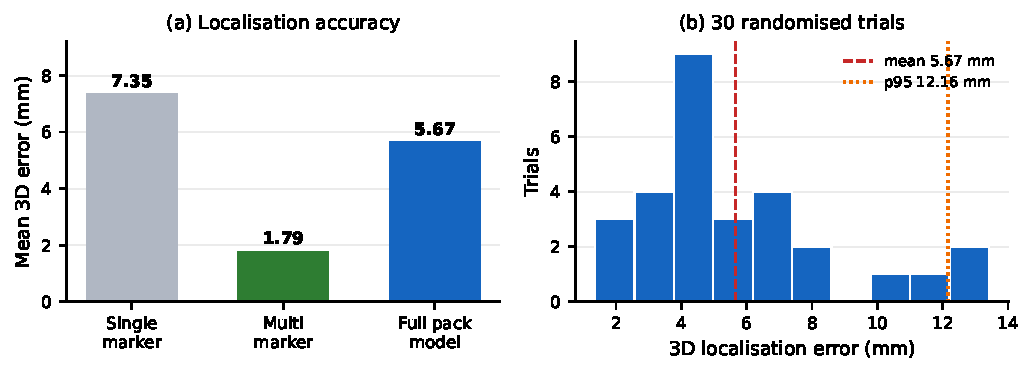
\includegraphics[width=\columnwidth]{figures/fig_localisation.pdf}
\caption{Monocular localisation accuracy. (a) Joint multi-marker estimation cuts
error by 75.6\% over a single marker; the full pack model is harder than primitive
geometry but stays under 6\,mm. (b) Error distribution over 30 randomised trials on
the pack model.}
\label{fig:loc}
\end{figure}

\begin{figure}[t]
\centering
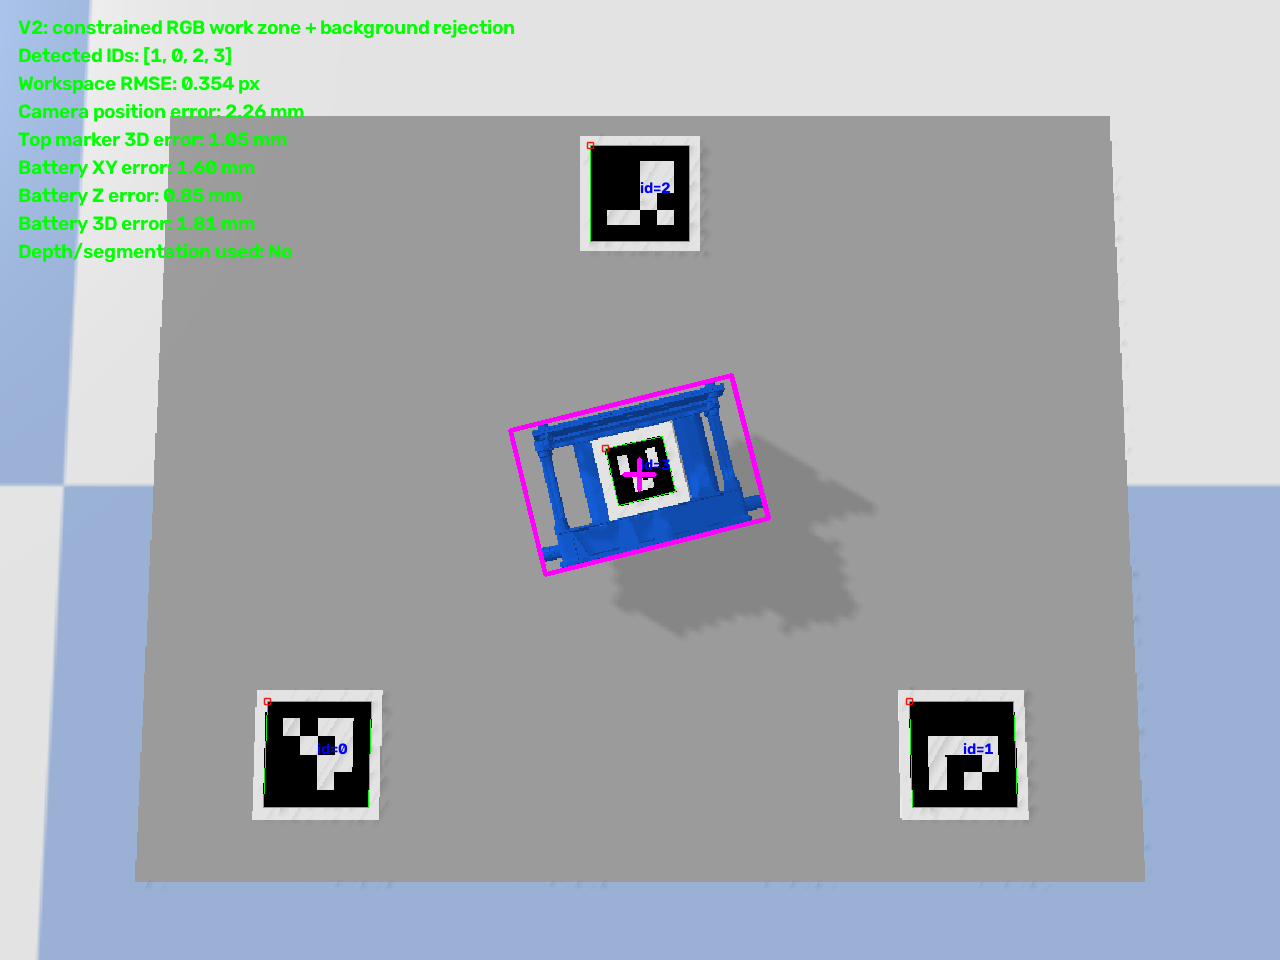
\includegraphics[width=0.86\columnwidth]{figures/fig_aruco_scene.png}
\caption{Localisation scene. Workspace markers (IDs 0--2) fix the metric reference
frame; the pack is found by the RGB detector (magenta) and never carries a marker
used as an object label. Workspace reprojection RMSE 0.354\,px.}
\label{fig:arucoscene}
\end{figure}

The residual error budget is informative: camera position error was 2.26\,mm and
workspace reprojection RMSE 0.354\,px, so a substantial part of the 5.67\,mm total is
attributable to the reference frame rather than to the detector. Improving marker
placement and calibration is therefore a more productive target than improving
detection precision, which is not obvious a priori.

Placing this alongside the manipulation literature: RAPID reports 0.9757 mAP@50 yet
57\% one-shot grasp success \cite{rapid2026}, indicating that the loss occurs between
perception and actuation. A 5.67\,mm target with a 12.16\,mm 95th percentile is
within the closing tolerance of a compliant gripper on a module of this scale,
suggesting the monocular route is viable for coarse positioning with final alignment
delegated to force feedback or visual servoing.

\subsection{Deployment}
INT8 quantisation of the detector to ONNX reduced latency by 20\% and model size by
46\% (44.8\,ms, 3.4\,MB on CPU) for a loss of 0.007 mAP@50, which is compatible with
edge deployment on a disassembly cell. The localisation stage adds only marker
detection and a PnP solve, both negligible against detector inference.

\subsection{Negative results}
\label{sec:negative}

We report failures that constrain the design space:

\begin{itemize}
\item \textbf{Open-vocabulary detection is unusable here.} YOLO-World, prompted with
``ev battery module'' and ``busbar'', scored 0.004 mAP@50 on the cross-facility test.
Battery internals are too far out of distribution for current open-vocabulary
detectors, notwithstanding their strong general-domain results.
\item \textbf{Naive multi-source merging degrades accuracy.} Merging all sources
without reconciling conventions reduced module mAP@50 to 0.331, below the
single-source baseline. More data reduced accuracy.
\item \textbf{Few-shot diffusion damage synthesis failed.} A LoRA-fine-tuned
inpainting model trained on six real damaged packs produced 180 crops that all
reproduced a memorised surface artefact rather than plausible damage. Below some
diversity threshold, generative augmentation reproduces incidental features.
\item \textbf{Copy-paste and glare augmentation reduced detector mAP} in our setting,
despite being widely reported as beneficial elsewhere.
\end{itemize}

\section{Limitations}

Our claims are about perception. We report metric localisation accuracy, not grasp
success: no physical manipulator was driven from these estimates, and as RAPID's 57\%
one-shot grasp rate at 0.9757 mAP@50 shows \cite{rapid2026}, perception accuracy does
not translate directly into manipulation success. Hand-eye calibration error, gripper
compliance and contact dynamics are outside our scope.

The localisation results are obtained in simulation. Simulation isolates the geometry
of the estimator from sensor noise, which is what we set out to measure, but it omits
motion blur, rolling shutter, marker occlusion by the manipulator, and the specular
highlights that make real battery internals difficult. Real-camera validation is
required before these figures can be claimed for a deployed cell, and we expect
degradation. The method also assumes packs rest on a support of known height; stacked
or tilted packs violate this and would require depth or a second view.

The condition-assessment test set is small (48 images, 14 damaged), so those figures
carry wide confidence intervals and should be read as indicative. Damaged-module
labels in public data are also of uncertain provenance: on inspection, several crops
labelled ``damaged'' showed no visible external damage, suggesting labels derived
from pack-level provenance rather than per-module inspection.

Finally, our data is assembled from public sources rather than collected under
controlled conditions, so pack-type coverage is uneven.

\section{Conclusion}

Single-facility evaluation substantially overstates how well EV battery module
detectors will perform in a recycling facility: a detector scoring 0.818 mAP@50
in-domain scored 0.277 across ten pack sources. Multi-source training with a frozen
DINOv2 backbone raises cross-facility accuracy to 0.502 mAP@50, and we showed that
this advantage is specifically robustness to annotation-convention shift rather than
better detection of conventional modules. We identified annotation convention as a
dominant and measurable failure mode, with per-source module mAP@50 ranging from
0.995 to 0.043. For condition assessment, a good-only anomaly detector matched
supervised recall (0.857) using no damaged training examples.

We then closed the loop from pixels to metres without a depth sensor. A
fiducial-referenced monocular transform localised a real pack model to 5.67\,mm mean
3D error over 30 randomised trials at a 96.7\% success rate, and solving jointly over
several markers rather than one reduced error by 75.6\%. Because most of the residual
budget traces to the reference frame rather than to detection, calibration quality is
the more productive engineering target.

Future work is real-camera validation of the localisation stage, integration with a
manipulator under force feedback, and closing the label loop by combining worker
annotations with electrical measurements taken on the line, which would supply the
damage labels that public data lacks.

\section*{Data Availability}
Annotations (16,945 polygon masks), evaluation code and trained detector weights are
available at \url{https://github.com/Komil-jon/ev-battery-vision-pipeline}.

\begin{thebibliography}{00}

\bibitem{zang2024robotic} Y. Zang, M. Qu, D. T. Pham, R. Dixon, F. Goli, Y. Zhang,
and Y. Wang, ``Robotic disassembly of electric vehicle batteries: Technologies and
opportunities,'' \emph{Computers and Industrial Engineering}, vol. 198, 110727, 2024.

\bibitem{tan2025screws} M. Tan, J. Huang, X. Jiang, Y. Fang, Q. Liu, and D. T. Pham,
``Robotic removal and collection of screws in collaborative disassembly of
end-of-life electric vehicle batteries,'' \emph{Biomimetics}, vol. 10, no. 8, 553,
2025.

\bibitem{rapid2026} ``RAPID: Robotic agentic platform for intelligent electric
vehicle disassembly,'' \emph{arXiv:2603.18520}, 2026.

\bibitem{screwrcnn2021} ``Accurate screw detection method based on Faster R-CNN and
rotation edge similarity for automatic screw disassembly,'' \emph{International
Journal of Computer Integrated Manufacturing}, vol. 34, no. 11, 2021.

\bibitem{screwbatt2023} ``An accurate activate screw detection method for automatic
electric vehicle battery disassembly,'' \emph{Batteries}, vol. 9, no. 3, 187, 2023.

\bibitem{screwcompare2026} ``Comparative analysis of YOLO and Faster R-CNN models for
EV battery screw detection,'' \emph{International Journal of Advanced Manufacturing
Technology}, 2026.

\bibitem{cvmodule2023} ``Computer vision application for industrial Li-ion battery
module disassembly,'' \emph{Production Engineering}, 2023.

\bibitem{dinov2} M. Oquab \emph{et al.}, ``DINOv2: Learning robust visual features
without supervision,'' \emph{Transactions on Machine Learning Research}, 2024.

\bibitem{rfdetr} Roboflow, ``RF-DETR: A real-time detection transformer,'' 2025.

\bibitem{patchcore} K. Roth, L. Pemula, J. Zepeda, B. Sch\"olkopf, T. Brox, and
P. Gehler, ``Towards total recall in industrial anomaly detection,'' in
\emph{Proc. IEEE/CVF CVPR}, 2022.

\bibitem{yolo11} G. Jocher and J. Qiu, ``Ultralytics YOLO11,'' 2024.

\bibitem{aruco2014} S. Garrido-Jurado, R. Mu\~{n}oz-Salinas, F. J. Madrid-Cuevas, and
M. J. Mar\'{i}n-Jim\'{e}nez, ``Automatic generation and detection of highly reliable
fiducial markers under occlusion,'' \emph{Pattern Recognition}, vol. 47, no. 6,
pp. 2280--2292, 2014.

\end{thebibliography}

\end{document}
